\section{Case 1: Ulovlig fildeling på universitetsnettet til NTNU}
Her viser vi alle resultatene i de forskjellige 

\subsection{Problemforståelse}
For å få økt forståelse for problemet og samtidig lære mer om verktøyene i RCA\cite{RCA} valgte vi to verktøy til problemforståelsen. Flytdiagram ble valgt for å få en oversikt i hvordan personer laster ned ulovlig materiale og hvordan dette påvirker universitet. Kritisk hendelser verktøy ble brukt til å finne ut hva det er personer laster ned.  
\subsubsection{Flytdiagram}
Flytdiagrammet her viser det vi anser som et normalt hendelsesforløp til hvordan man laster ned materiale på universitetsnettverket. Det gjøres den antagelsen at private tjenester ikke er med i statistikken fra universitet og at det ikke kommer noen opphavsrettsnotiser fra brukere som bruker private tjenester. Med private tjenester mener vi lukkede nettsamfunn som bare er til for å distribuere opphavsrettsbeskyttet materiale gratis.

\begin{figure}[H]
    \centering
    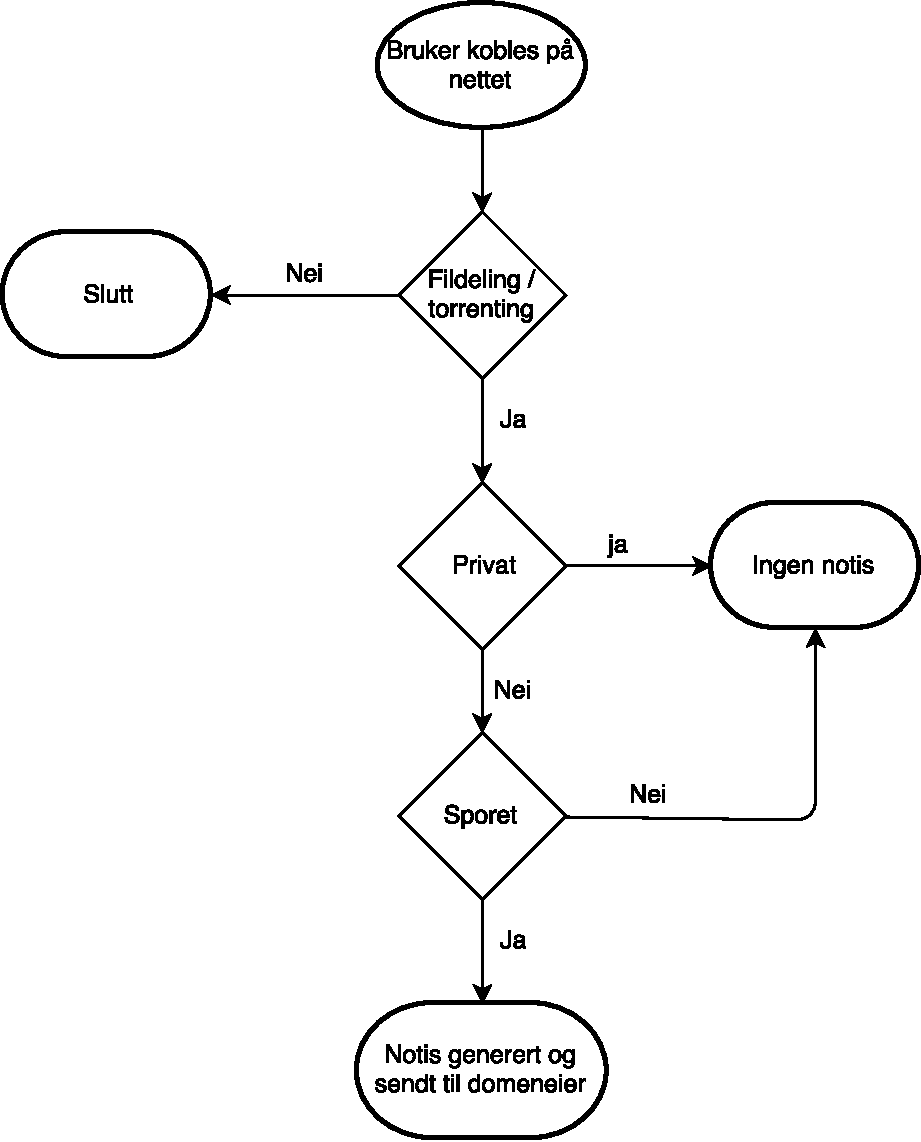
\includegraphics[scale=0.5]{case_1/bilder/Flowchart.pdf}
    \label{fig:Flytdiagram}
    \caption[Flytdiagram for fildeling]{Flytdiagram for fildeling}
\end{figure}

\subsubsection{Kritiske hendelser}
For å besvare hva som ble lastet ned brukte vi kritisk hendelse for å få et enkelt overblikk. Dette ble gjort på en veldig uformell måte, der vi spurte studenter som var i nærheten. Merk at hver person kan svare at de laster ned fra flere kategorier.


Spørsmål stilt til intervjuobjekter:
\begin{itemize}
    \item Bor du, eller har du bodd i SiT-bolig i løpet av studiet? (Hvis nei, avslutt intervju)
    \item Bruker du, eller har du brukt Torrents til å laste ned opphavsrettsbeskyttet materiale mens du bodde i SiT-bolig? Hvis ja, hvilke av følgende kategorier laster du ned fra? (Viser kategoriene)
\end{itemize}

\noindent Dette er resultatet fra spørringene: \\
\indent Antall spurt: 13 \\
\indent Antall som aldri laster ned: 4
\begin{table} [H]
    \begin{tabular}{ | m{20em} | m{20em} | }
        \hline
            \cellcolor{yellow} Fildelingskategori & \cellcolor{yellow} Frekvens \\
        \hline
            Filmer og serier & 8  \\
        \hline
            Spill & 3 \\
        \hline
            Skolebøker & 2 \\
        \hline
            Musikk & 2 \\
        \hline
            Programvare og bøker utenom skolebruk & 1 \\
        \hline
            Programvare til skolebruk & 0 \\
        \hline
            Annet & 0 \\
        \hline
    \end{tabular}
    \caption{Oversikt over kvantiteten av kritiske hendelser ved torrenting av opphavsrettsbeskyttet materiale}
    \label{kritisk_tabell_1}
\end{table}


\subsection{Idémyldring}
I idémyldring ble verktøyet idémyldring valgt da det fungerer godt for vår gruppe dynamikk 
\subsubsection{Idémyldring}
Etter idémyldringen var ferdig ble det gjort en vurdering av resultatene og de ble kategorisert i henhold til likhetstrekk, under en fellesnevner som for eksempel Økonomi. Resultater og gruppering er som vist i figur \ref{fig:idemyldring} under. Merk at noen årsaker kunne ikke plasseres i én kategori og er derfor direkte knyttet til problemstillingen. 

\begin{figure}[H]
    \centering    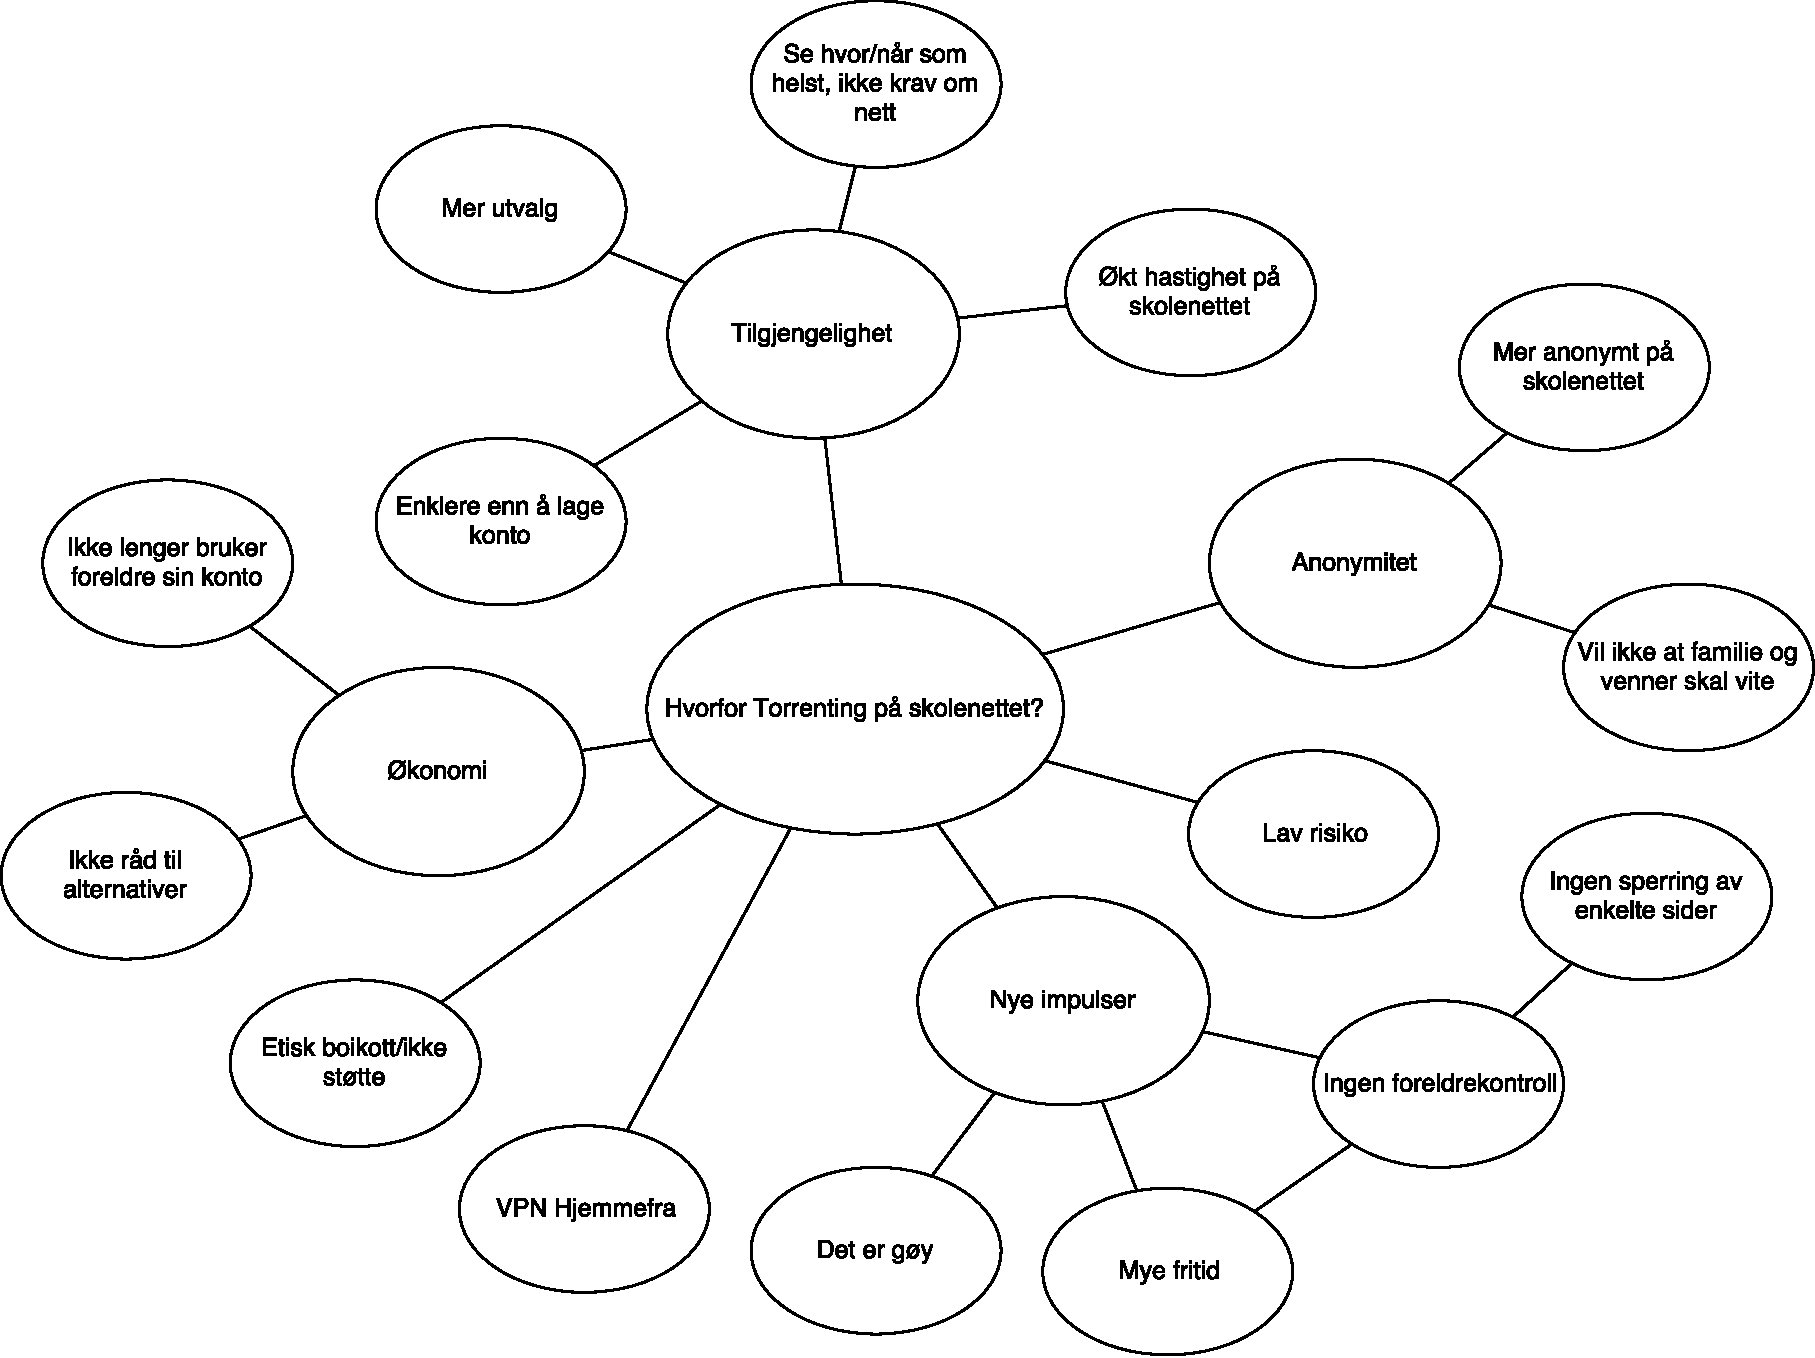
\includegraphics[scale=0.45]{case_1/bilder/idemyldring}
    \caption[Idémyldring]{Resultater og gruppering av idémyldringen}
    \label{fig:idemyldring}
\end{figure}

Resultatene er gruppert inn i fire hovedkategorier, Økonomi (som går på kjøpekraften til den enkelte person), Tilgjengelighet (hvor god tilgang en har på tjenester), Anonymitet (foreldre kunne blant annet overvåke før, samt føler seg tryggere når det er flere på samme nett) og nye impulser (mer frihet og fritid, og påvirkning av nedlastningskulturen).


\subsection{Datainnsamling}
Det var forskjellige metoder å drive med datainnsamling, vi valgte kvantitativ spørreundersøkelse for å spørre mest mulig beboere fra Sit. Undersøkelsen ble begrenset til Gjøvik og endte med 97 svar totalt, dette er 18.6\% av de 522 beboerne i Sit bolig. Av disse var det 34 som svarte at de hadde lastet ned opphavsrettsbeskyttet materiale i hybelen, det er 35\% av de spurte. 

Undersøkelsen ble sendt ut gjennom forskjellige facebook sider tilhørende studentenmiljø i Gjøvik. I tillegg til facebook ble en plakat laget og ble lagt i postkassen til cirka halvparten av studentboligen på Kallerud og Sørbyen. Etter at det hadde gått en uke oversatte vi spørreundersøkelsen til engelsk, der vi hadde en kommunikasjonskanal som kunne sende denne til de fleste internasjonale studentene, der mange av disse bor på Sit hybler. Vi fikk rundt 20 respondenter fra de internasjonale, og alle disse resultatene ble oversatt til norsk og lagt inn i et samlet spørreskjema. 

\subsection{Dataanalyse}
Vi brukte tre verktøy til dataanalysen der to var fra boken\cite{RCA} pluss en ANOVA analyse. ANOVA analyse ble gjort får å prøve litt forskjellige verktøy, men er lagt i vedlegg da analysen ikke førte til noe signifikant data. De to andre verktøyene er histogram for å få oversikt og affinitetsdiagram til å få sortert skriveoppgavene. Under viser hvor mange som laster ned av de 97 som ble spurt i prosent. Rundt 37\% sier at det laster ned, som er en stor del av studentmassen. Det kan ha en påvirkning at undersøkelsen har en overvekt av studentene kommer fra informatikk- og datarelaterte studier.  


\begin{figure}[H]
    \centering
    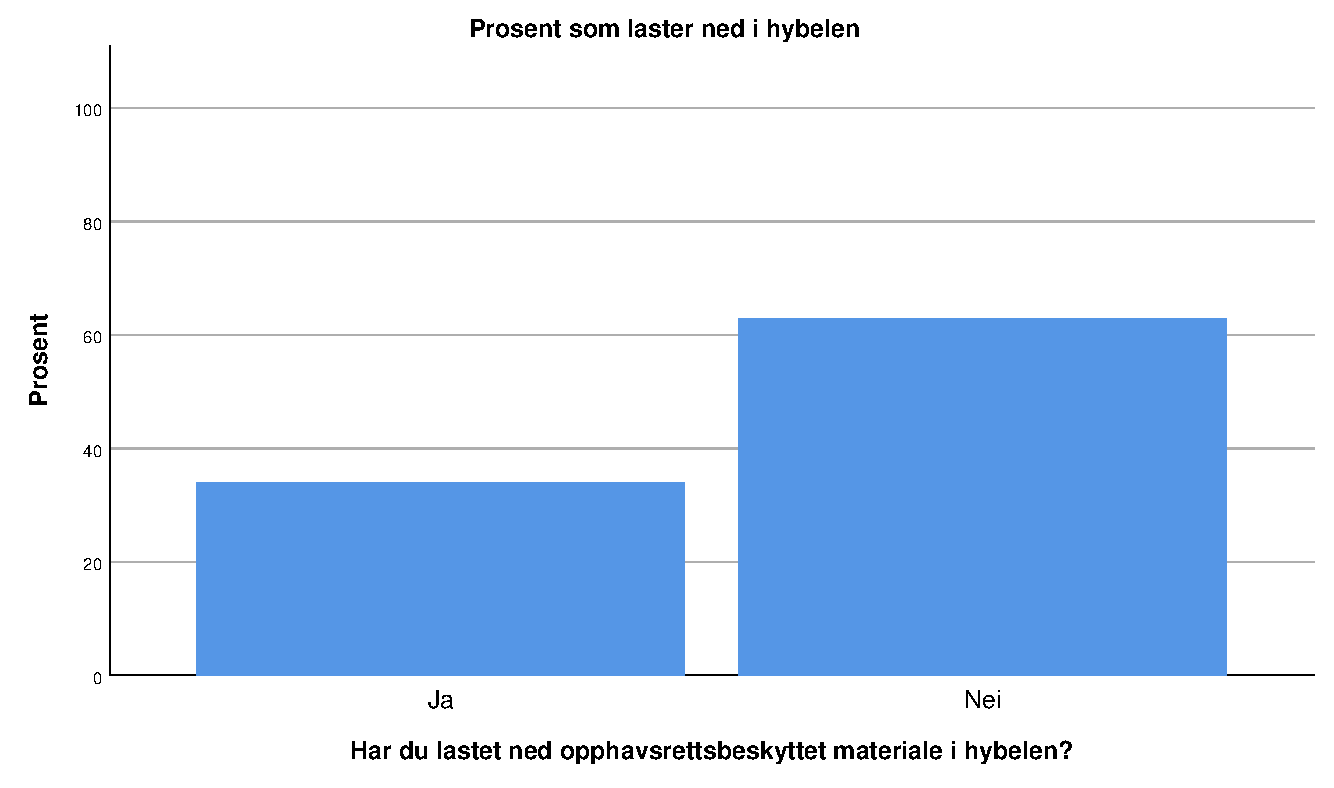
\includegraphics[scale=0.45]{case_1/bilder/lasterned.pdf}
    \label{fig:lasterned}
    \caption[Laster ned]{Hvor mange som laster ned av de spurte}
\end{figure}


\subsubsection{Kjønnsforskjeller}
Vi ønsket også å undersøke om det er noen forskjeller i hvem som laster ned basert på kjønn. Under ser vi forholdet mellom kjønnene.
\begin{figure}[H]
    \centering
    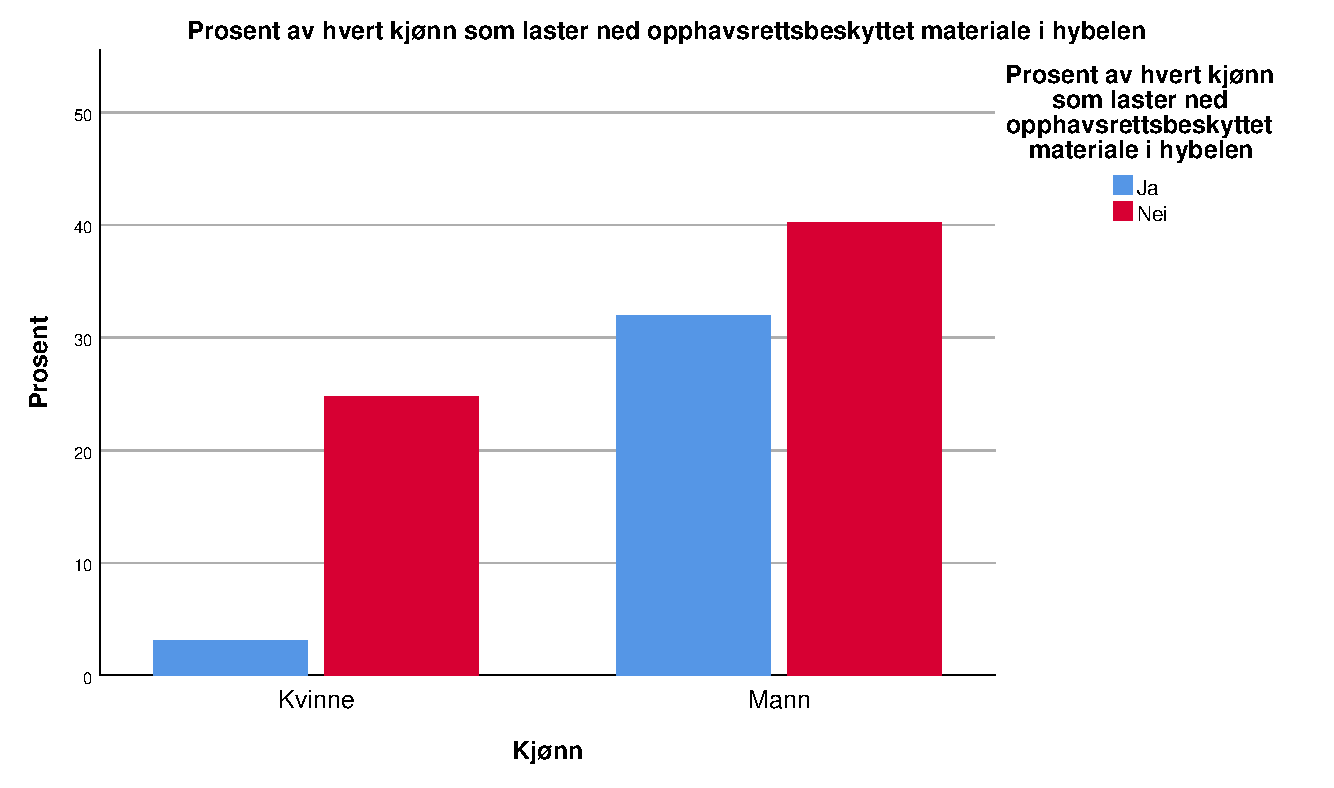
\includegraphics[scale=0.45]{case_1/bilder/kjonn_lasterned.pdf}
    \label{fig:kjønn_lasterned}
    \caption[Kjønn laster ned]{Hvor mange fra hvert kjønn som laster ned}
\end{figure}
Vi kan se over at det er i hovedsak menn som laster ned ulovlig, mens kvinner har svart at de i stor grad ikke laster ned. Dette blir selvfølgelig påvirket at det er få kvinner i IT-relaterte studier, som vi har funnet ut at utgjør noe mer av nedlastingen. Det er derimot vanskelig å vite helt sikkert om det er fordi kvinner er underrepresentert i IT studier som gir utslag, eller om det er kvinner generelt sett som ikke laster ned. Der er likevel en mer signifikant forskjell mellom kjønnene enn det er mellom IT studier og andre studier som vist i figur \ref{fig:IT-lasterned}, så vi velger å tolke det som at kvinner laster ned mindre enn menn.


\begin{comment}


\subsubsection{Forskjeller mellom studentbyer}
Samtlige studentbyer har et kablet nettverk av Uninett godt egnet for nedlasting, enten det er lovlig eller ulovlig nedlasting. Det er derimot noen forskjeller i hastighet på enkelte studentbyer. Nordbyen, Sørbyen og Sentrum har muligheten til 100Mbps nedlasting og 100Mbps opplasting, mens Kallerud har en øvre grense på hele 1000Mbps nedlasting og 1000Mbps opplasting. Dette er ti ganger hastigheten til de andre studentbyene. Derfor ønsket vi å undersøke om dette hadde noe relevans i forhold til hvor mange som laster ned ulovlig. 

\begin{figure}[H]
    \centering
    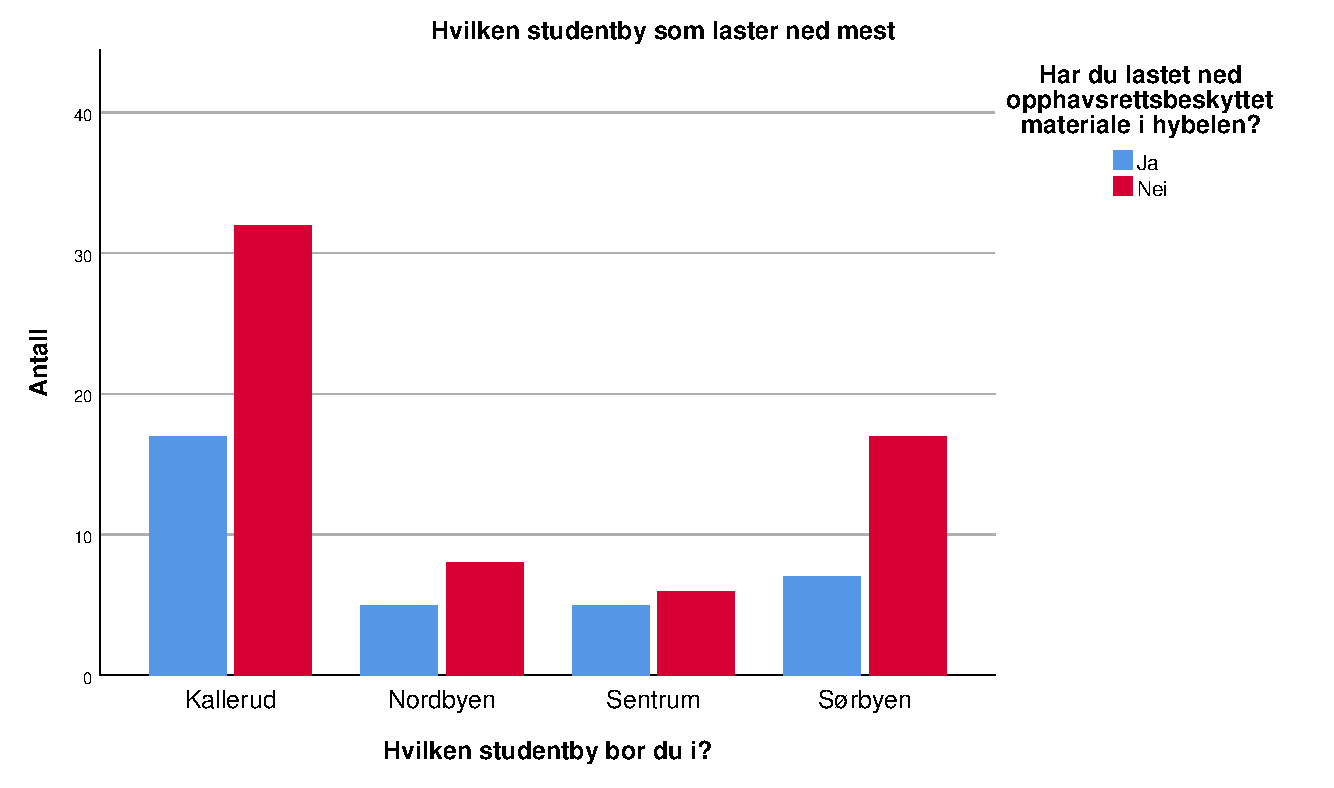
\includegraphics[scale=0.45]{case_1/bilder/studentby_lasterned.pdf}
    \label{fig:studentby_lasterned}
    \caption[Studentby laster ned]{Hvor mange fra hver studentby som laster ned}
\end{figure}

På grunn av lav oppslutning på Nordbyen og Sentrum er det vanskelig å si noe sikkert på dem, mens Kallerud og Sørbyen ikke varierer så veldig fra hverandre. Når vi bruker histogrammer ser vi ingen signifikant forskjell mellom studentbyene når det kommer til nedlasting som vi kan si med sikkerhet.



\end{comment}

\subsubsection{Konsekvenser ved nedlasting}
Et spørsmål som ble spurt i spørreundersøkelsen var hvor godt kjent de var med mulige konsekvenser ved ulovlig nedlasting, og med det brudd på opphavsretten. Det kunne være relevant å se om det var noen spesiell sammenheng mellom de som ikke kjente til konsekvensene og de som lastet ned. 

\begin{figure}[H]
    \centering
    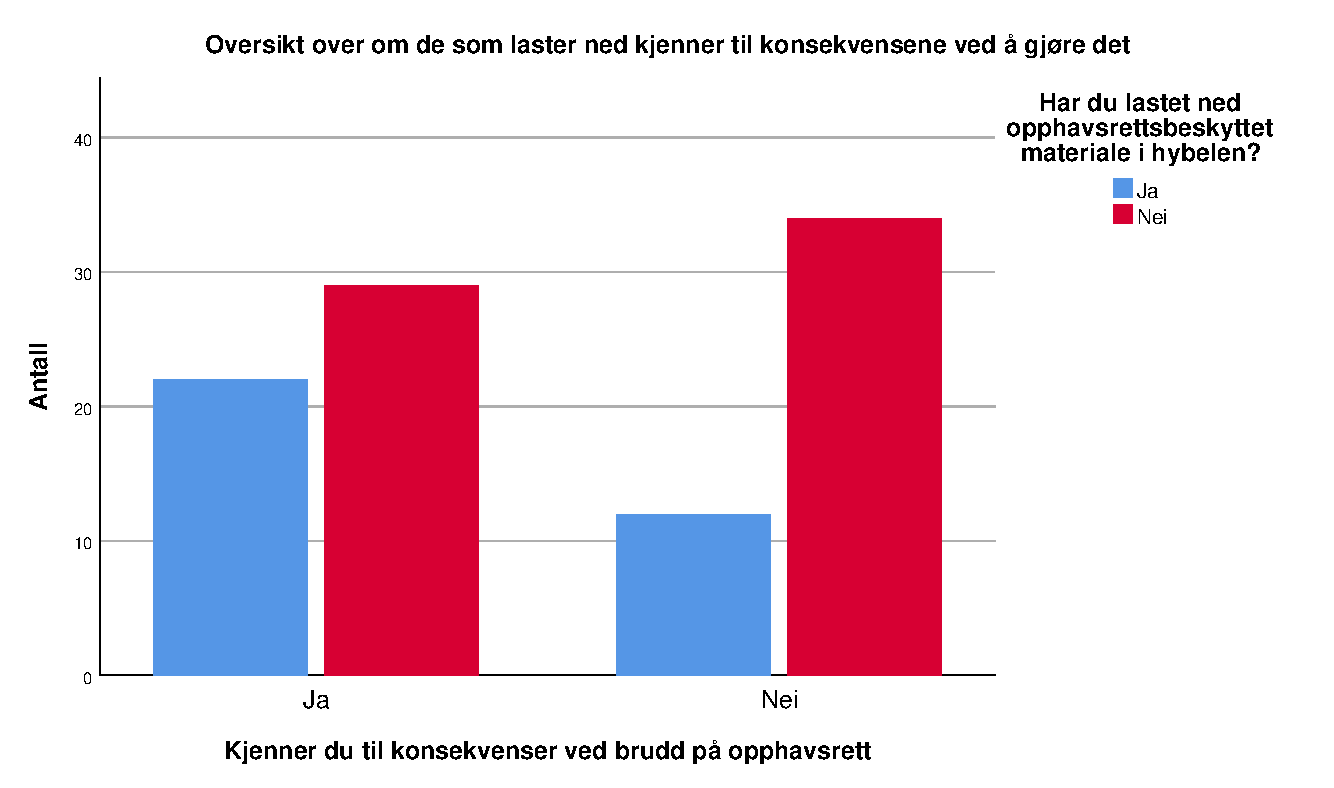
\includegraphics[scale=0.45]{case_1/bilder/konsekvens_lasterned.pdf}
    \label{fig:konsekvens_lasterned}
    \caption[Konsekvens av å laste ned]{Hvor mange som kjenner til konsekvenser ved å laste ned}
\end{figure}

Det viser seg faktisk at de som laster ned har en bedre kjennskap til konsekvensene enn de som ikke gjør det. Det kan kanskje ha noe å gjøre med at de er mer opptatt av problemområdet enn de som ikke laster ned. De som ikke laster ned i første omgang har kanskje ingen grunn til å sjekke konsekvensene av det. I tillegg fant vi ut at IT-studenter kjenner konsekvenser bedre enn de andre, og de har også høyere andel nedlastere. Vi prøvde å kjøre samme test på hvor godt de kjenner til IT-reglementet til NTNU \cite{ITReg} og kom til samme konklusjon som over. Dette histogrammet kan sees \hyperref[fig:reglement-lasterned]{her}. En grunn til dette er også igjen at IT-studenter kjenner bedre til IT reglementet, som vist \hyperref[fig:reglement-fakultet]{her}, og de er i overvekt. Så dette må tas i betraktning. 

En mulig teori vi ønsket å prøve ut var om mange som lastet ned ikke kjente til konsekvensene ved ulovlig nedlasting eller NTNU sitt IT-reglementet, og lastet ned på grunn av det. Dette ble altså delvis motbevist.

\subsubsection{Årsaker til nedlasting}
I spørreundersøkelsen kom vi med seks påstander til hvorfor respondentene laster ned, som de besvarte på en likert-skala fra 1 til 5, der 1 er i liten grad og 5 er i stor grad. Etter å ha analysert alle seks påstandene ved hjelp av SPSS og histogrammer fant vi én påstand som hadde en graftopp der respondentene svarte positivt. De aller fleste svarte de var enige i at de lastet ned på grunn av tilgjengelighet.

\begin{figure}[H]
    \centering
    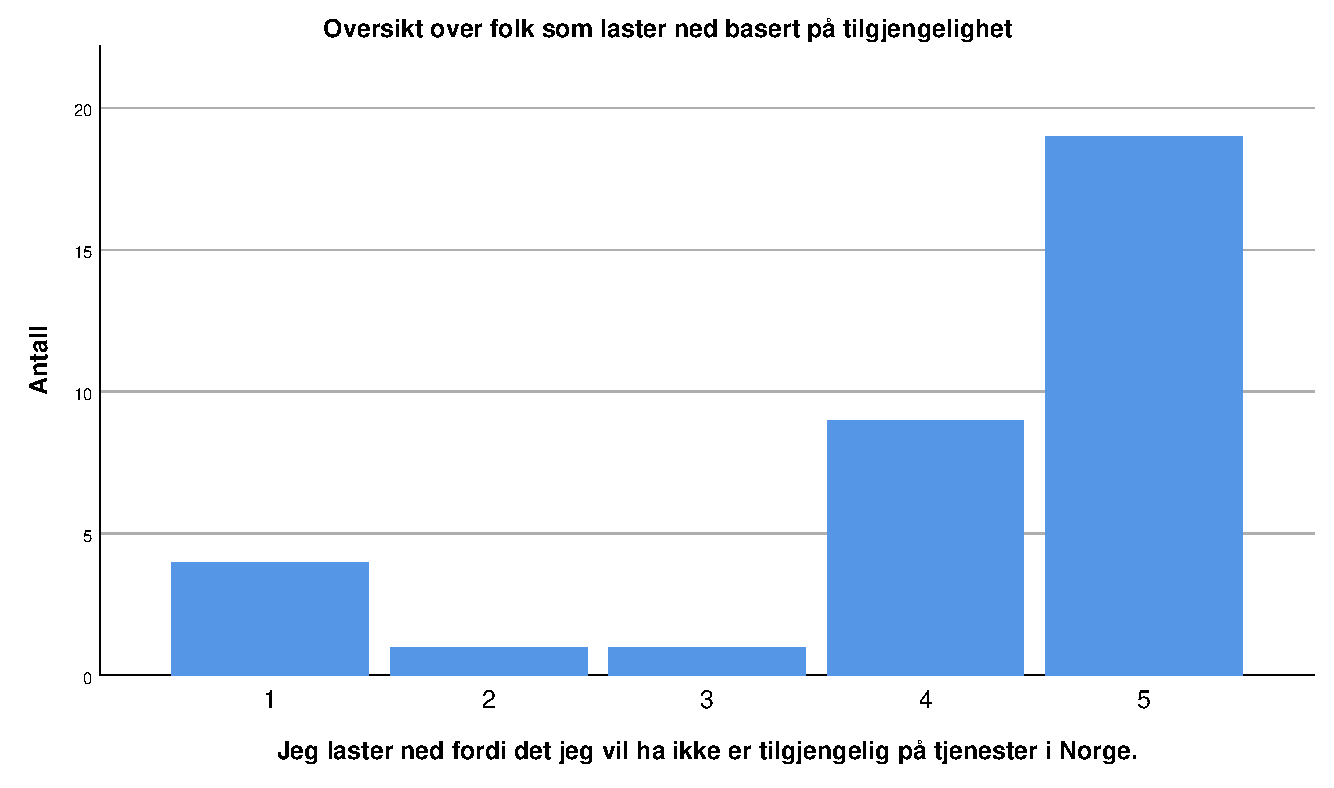
\includegraphics[scale=0.45]{case_1/bilder/tilgjengelighet.pdf}
    \label{fig:tilgjengelighet}
    \caption[Tilgjengelighet]{Hvor mange som laster ned av de spurte}
\end{figure}

Dette vil si at det er godt mulig at tilgjengeligheten er en årsak til om en laster ned eller ikke, og er verdt å dokumentere til videre analyse. Siden tilgjengelighet betyr så mye, var det naturlig å utforske det ytterligere. Vi fant ut at det kunne være relevant å vite om de som brydde seg om tilgjengelighet hadde tilgang på strømmetjenester, og i så fall hvor mange.

\begin{figure}[H]
    \centering
    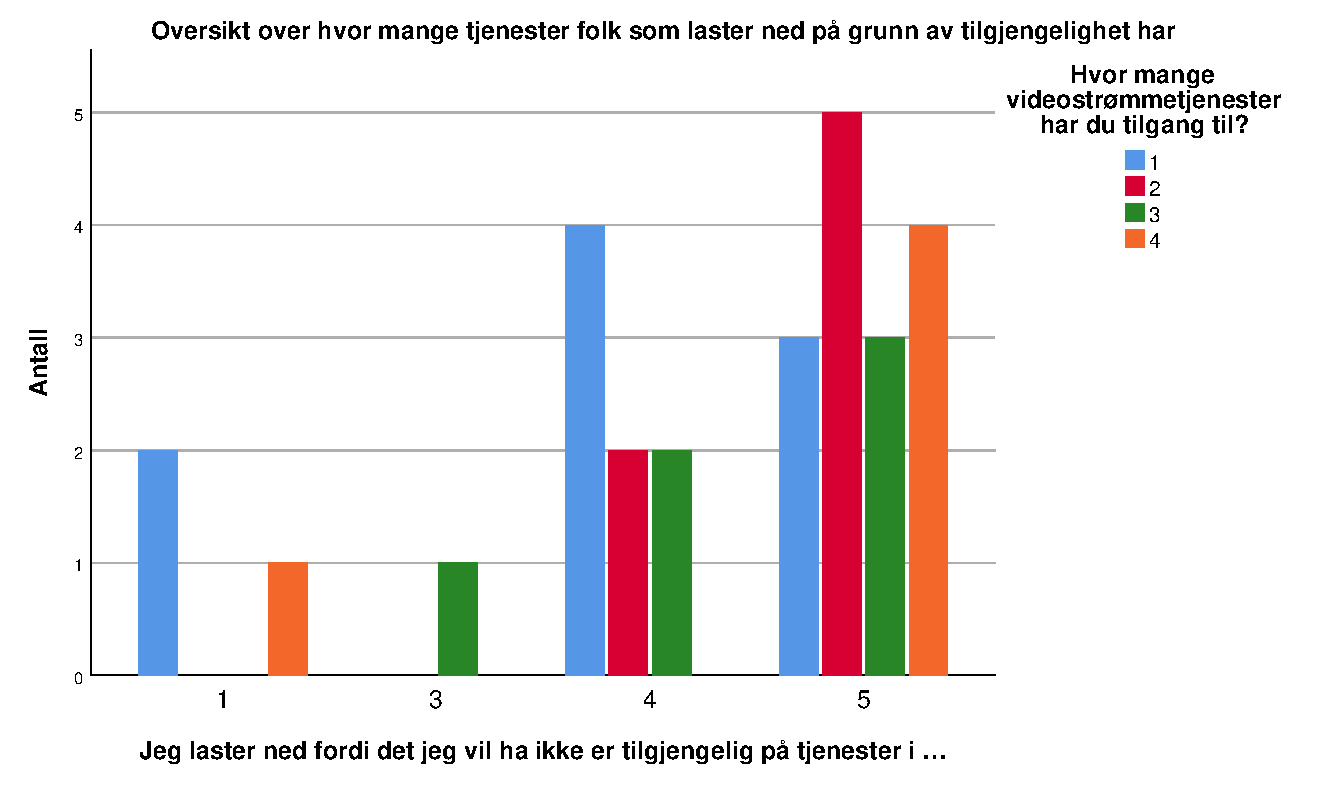
\includegraphics[scale=0.45]{case_1/bilder/tilgjengelighet_antallstromming.pdf}
    \label{fig:tilgjengelighet_antallstromming}
    \caption[Tilgjengelighet vs antall strømmetjenester]{Korrelasjonen mellom de som laster ned på grunn av tilgjengelighet og hvor mange tjenester de har tilgang på}
\end{figure}

Her viser det seg at de som laster ned på grunn av tilgjengelighet også har en god del strømmetjenester. Dette sier at mange av disse er storforbrukere av film og serier, og at det ikke har så mye å si om de har tilgang til tjenestene eller ikke. Dette vil muligens utelukke en løsning i form av at NTNU tilbyr en tjeneste siden de kommer til å laste ned uansett.

%--------------------------------------------------------








\begin{comment}
Her nevner vi kort våre resultater i de viktigste fasene som hadde direkte innvirkning på identifisering og eliminering av rotårsaken. 

\subsection{Datainnsamling}
Det var forskjellige metoder å drive med datainnsamling, vi valgte kvantitativ spørreundersøkelse for å spørre mest mulig beboere fra Sit. Vi fikk svarprosent på ca 18\%, og vi forventet svarprosent på 15-20\% av alle beboere i Sit boligene i Gjøvik. Vi valgte å forholde oss til studentbyene i Gjøvik, ikke i Trondheim eller Ålesund. Av studentbyene vi spurte, fikk vi desidert mest svar fra Kallerud. Av alle som svarte var det 50\% som bodde på kallerud

Vi postet et innlegg på Huset ansatte, og tok kontakt med linjeforeningene der vi spurte om de kunne legge ut en link til undersøkelsen. Her fikk vi best respons fra Huset ansatte og INGa sine facebooksider. Vi la også en plakat i litt under halvparten av postkassene på Kallerud og på Sørbyen, og vi fikk grei respons fra dette.

Etter at det hadde gått en uke oversatte vi spørreundersøkelsen til engelsk, der vi hadde en kommunikasjonskanal som kunne sende denne til alle de internasjonale studentene, der mange av disse bor på Sit hybler. Vi fikk rundt 20 respondenter fra de internasjonale, og alle disse resultatene ble oversatt til norsk og lagt inn i et samlet spørreskjema.


\subsection{Dataanalyse}
Kartlegging av omfanget viste at 35\% av de spurte drev med ulovlig fildeling. Dette var lavere enn vi trodde, men fortsatt mange. De fleste var småforbrukere, men det var også en del storforbrukere som laster ned over ti torrents i måneden. Fra dataanalysen kunne vi også konkludere med at tilgjengelighet var en svært viktig grunn til at folk lastet ned. Selv de som hadde tilgang på mange strømmetjenester svarte at tilgjengeligheten var en viktig grunn til at de lastet ned. Økonomi var viktig for noen, men også uviktig for en god del. Det viste seg også at det var dårlig håndhevelse og kommunikasjon av lover og regler. 

Det var også forskjeller blant demografiene. Menn var en stor andel av de som lastet ned, mens kvinner nesten ikke lastet ned noe. Når det kommer til fakultet var IT fakultetet overrepresentert i nedlastingsstatistikken. De var også de som kjente til IT reglement og konsekvenser best. Generelt sett var det lite kunnskap om IT reglement, og varierende kjennskap til konsekvenser. 

\subsection{Rotårsaksidentifisering}
Vi valgte å bruke fiskebein for å strukturerte vår rotårsaksidentifisering. Som et verktøy fungerte det meget godt, der vi klarte å få organisert årsakene inn i tre hovedgrupper: Økonomi, Tilgjengelighet og Risiko. Vi analyserte hver hovedgruppe nøyere og kom fram til en årsak for hver gruppe: Dårligere utvalg på alternative tjenester i Norge, Tjenestene er ikke verdt prisen og Håndheving og kommunisering av lovene knyttet til ulovlig fildeling blir ikke prioritert. 

\subsection{Rotårsakseliminering}
Det vi kom frem til her var fire forskjellige løsninger for å fjerne rotårsaken, der to av dem var mer globale og ikke gjennomførbare for skolen, og to mer praktisk gjennomførbare som ikke fjerner det at folk laster ned, men skyver problemet over til andre. De ikke gjennomførbare var at alt av materiale blir gratis og tilgjengelig på ett samlet sted, og fjerne de geografiske blokkeringene. De gjennomførbare var at man bytter ISP til studentboligene for å forflytte problemet bort fra NTNU's ansvarsområde, og stenge torrentprotokollen for alle på nettverket. 

\subsection{Løsningsimplementering}
Vi benyttet trediagram (figur \ref{fig:Tre-diagram}) for å illustrere de ulike arbeidsoppgavene som kreves for å implementere tiltakene.
\end{comment}